\documentclass[11pt]{beamer}
\usetheme{Warsaw}
\usepackage[utf8]{inputenc}
\usepackage[french]{babel}
\usepackage[T1]{fontenc}
\usepackage{fancyref}
\usepackage{natbib}
\usepackage[utf8]{inputenc}
\usepackage[french]{babel}
\usepackage[T1]{fontenc}
\usepackage{amsmath}
\usepackage{amsfonts}
\usepackage{amssymb}
\usepackage{graphicx, float}
\usepackage{algorithm, algorithmic}
\usepackage{csquotes}
\usepackage{wasysym}
\usepackage{dsfont}
\usepackage{yhmath}
\usepackage{textcomp}
\usepackage{eurosym}

\usepackage{hyperref}
\usepackage{tabularx}
\usepackage{colortbl}
\usepackage{hhline}


\newcommand{\lexp}[1]{\phantom{}^{#1}}
\newcommand{\elem}[4]{\lexp{#2}#1^{#3}_{#4}}

\author{Guillaume Rochette}
\title{Stage de Fin d'Études
		\\
Création d'un Moteur de Recherche dans les Images Satellite}
\date{\today}
\setbeamertemplate{footline}[frame number]

\begin{document}

\begin{frame}
\titlepage
\end{frame}

\begin{frame}{Le Groupe Thales}
	\begin{figure}[H]
		\centering
		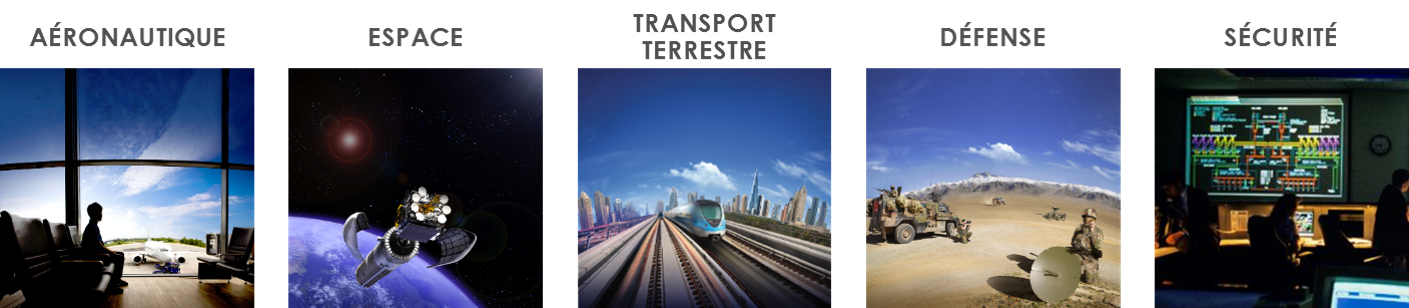
\includegraphics[scale=0.425]{Images/Secteurs_Activites.png}
		\caption{Secteurs d'activités du Groupe Thales}
	\end{figure}
	Présent dans 56 pays, employant 64000 salariés, dont 34000 en France.
	\begin{itemize}
		\item Présence dans 56 pays.
		\item 64000 salariés, dont 34000 en France.
		\item 15 Mds€.
	\end{itemize}
\end{frame}

\begin{frame}{Thales Services}
	Thales Services est une entreprise spécialisée dans les activités de conception, développement et maintenance de systèmes informatiques sécurisés.
	\begin{figure}[H]
		\centering
		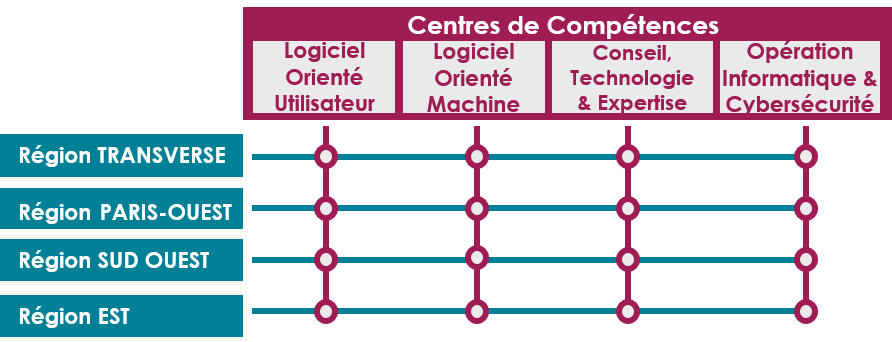
\includegraphics[scale=0.55]{Images/Matrice_Thales_Services.png}
		\caption{Organisation matricielle de Thales Services}
	\end{figure}
	Ce stage s'effectue dans le \emph{Centre de Compétences} \textbf{Logiciel Orienté Machine} de la \emph{Région Sud-Ouest}.
\end{frame}

\begin{frame}{Objectifs du Stage}
	\begin{itemize}
		\item Apporter des connaissances relatives à l'apprentissage profond appliqué au traitement de l'image.
		\item Déterminer des opportunités d'application de vision par ordinateur pour des images satellite, telle que de la segmentation d'image ou de la recherche de similarités.
		\item Proposer et évaluer des modèles pour les applications proposées.
	\end{itemize}
\end{frame}
\begin{frame}{L'Apprentissage Machine}
	\begin{displayquote}
		On dit qu'un algorithme apprend grâce à une expérience \emph{E}, par rapport à une classe de tâches à accomplir \emph{T}, dont on peut calculer la mesure de performance \emph{P}, si sa capacité d'accomplir la tâche \emph{T}, mesurée par la performance \emph{P}, s'améliore avec l'expérience \emph{E}.
	\end{displayquote}
	\begin{flushright}
		T.M. Mitchell
	\end{flushright}
	\begin{itemize}
		\item Tâche : Classification, Régression, etc.
		\item Mesure de Performance : Distance Euclidienne, Entropie Croisée, etc.
		\item Expérience : Nature des Données, Apprentissage Supervisé/Non-Supervisé, etc.
	\end{itemize}
\end{frame}

\begin{frame}{Optimisation et Régularisation}
	\begin{block}{Optimisation}
		Minimisation de la Fonction de Perte $\rightarrow$ Problème d'Optimisation.
		
		Utilisation de Méthodes de Descente de Gradient.
	\end{block}
	\begin{block}{Régularisation}
		Rasoir d'Ockham :
		\begin{displayquote}
			Les hypothèses suffisantes les plus simples sont les plus vraisemblables.
		\end{displayquote}
		\begin{figure}[H]
			\centering
			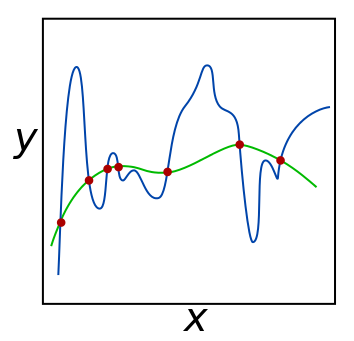
\includegraphics[scale=0.325]{Images/Regularization.png}
		\end{figure}
	\end{block}
\end{frame}

\begin{frame}{Neurone}
Un neurone artificiel est une application $f : \mathbb{R}^p \rightarrow \mathbb{R}$, paramétrée par $\theta = (b,w) = (b, w_1, ..., w_p)$, le biais et les poids.
\begin{figure}[H]
	\centering
	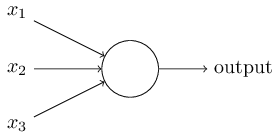
\includegraphics[scale=0.6]{Images/Neuron.png}
	\caption{Schéma d'un Neurone}
\end{figure}
La sortie du neurone :
$$a = g(w^Tx + b)$$
\end{frame}

\begin{frame}{Réseau de Neurones}
\begin{figure}[H]
	\centering
	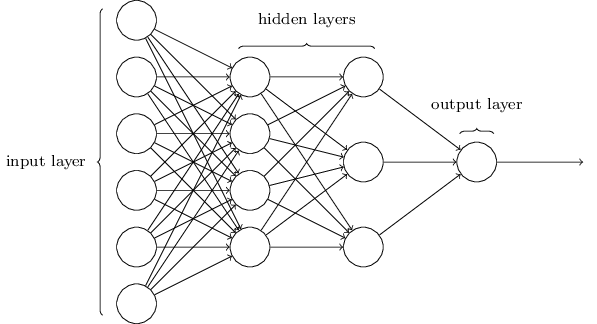
\includegraphics[scale=0.5]{Images/Neural_Network.png}
	\caption{Schéma d'un Réseau de Neurones}
\end{figure}
\end{frame}

\begin{frame}{Propagation}
	\begin{algorithm}[H]
		\caption{Algorithme de Propagation}
		\begin{algorithmic}
		    \REQUIRE {
		    Un réseau de neurones de $L$ couches, défini par $S = (S_1, S_2, ..., S_L)$.\\
		    Un vecteur d'entrée $x \in \mathbb{R}^n = \mathbb{R}^{S_1}$,\\
		    $\ $\\
		     }
		    \STATE $\elem{a}{0}{}{} = x$
		    \FOR{$k=1$ \TO $L$}
		    	\STATE $\elem{z}{k}{}{} = (\elem{w}{k}{}{})^T(\elem{a}{k-1}{}{}) + \elem{b}{k}{}{}$
		    	\STATE $\elem{a}{k}{}{} = g(\elem{z}{k}{}{})$
		    \ENDFOR
		    \RETURN $\elem{a}{L}{}{}$
		\end{algorithmic}
	\end{algorithm}
\end{frame}

\begin{frame}{Rétro-propagation}
	\begin{algorithm}[H]
		\caption{Algorithme de Rétro-propagation}
		\begin{algorithmic}
		    \REQUIRE {
		    Un réseau de neurones de $L$ couches, défini par $S = (S_1, S_2, ..., S_L)$.\\
		    $x \in \mathbb{R}^n = \mathbb{R}^{S_1}$, $y \in \mathbb{R}^m = \mathbb{R}^{S_L}$.\\
		    $\ $\\
		     }
		    \STATE $\elem{\delta}{L}{}{} = \nabla_{\elem{a}{L-1}{}{}} C$
		    \STATE $\nabla_{\elem{b}{L}{}{}} C = \elem{\delta}{L}{}{}$
		    \STATE $\nabla_{\elem{w}{L}{}{}} C = \elem{\delta}{L}{}{} \times{\elem{a}{L-1}{}{}}^T $
		    
		    \FOR{$k=L-1$ \TO $1$}
		    	\STATE $\elem{\delta}{k}{}{} = ((\nabla_{\elem{a}{k}{}{}}\elem{z}{k+1}{}{})^T \times \elem{\delta}{k+1}{}{}) \odot \nabla_{\elem{z}{k}{}{}}{\elem{a}{k}{}{}}$
		    	\STATE $\nabla_{\elem{b}{k}{}{}} C = \elem{\delta}{k}{}{}$
		    	\STATE $\nabla_{\elem{w}{k}{}{}} C = \elem{\delta}{k}{}{} \times{\elem{a}{k-1}{}{}}^T $
		    \ENDFOR
		\end{algorithmic}
	\end{algorithm}
\end{frame}

\begin{frame}{Convolution}
	Expression générale :
	$$(I*K)_{i,j} = \sum_{m}\sum_{n}{I_{m,n}K_{i-m,j-n}}$$
	\begin{figure}[H]
		\centering
		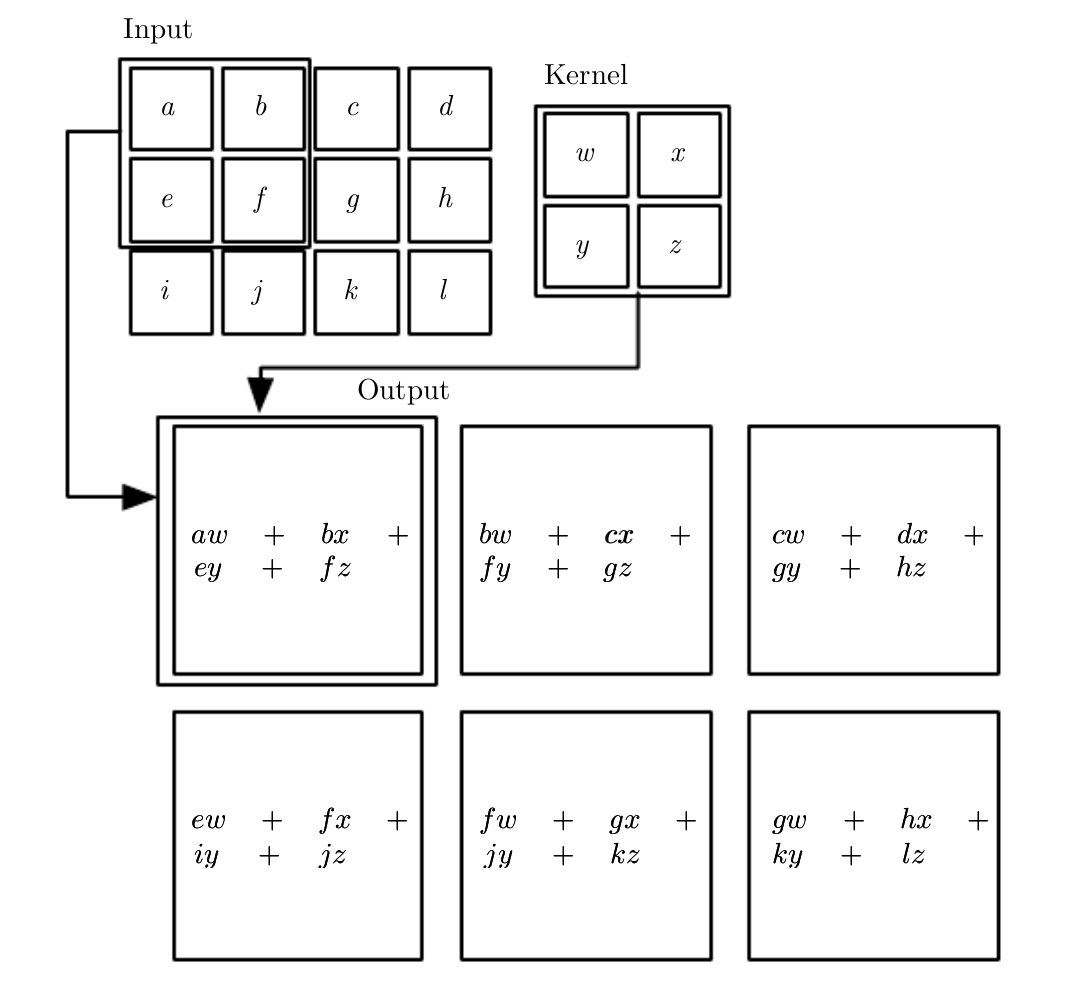
\includegraphics[scale=0.175]{Images/Convolution.png}
	\end{figure}
\end{frame}
\begin{frame}{Intérêts}
	\begin{itemize}
		\item Interaction locale.
		\item Partage des paramètres.
		\item Invariance par translation.
	\end{itemize}
\end{frame}

\begin{frame}{Réduction de la Dimensionnalité}
	Problème : Classifier des images de dimensions $(3, 256, 256)$ en $1000$ catégories.
	
	\emph{À noter :} $3 \times 256 \times 256 = 196608$.
	
	\begin{center}
		Comment extraire de l'information pertinente à partir de ces $196608$ variables ?
	\end{center}
\end{frame}
\begin{frame}{Approche Naïve}
	\begin{figure}[H]
		\centering
		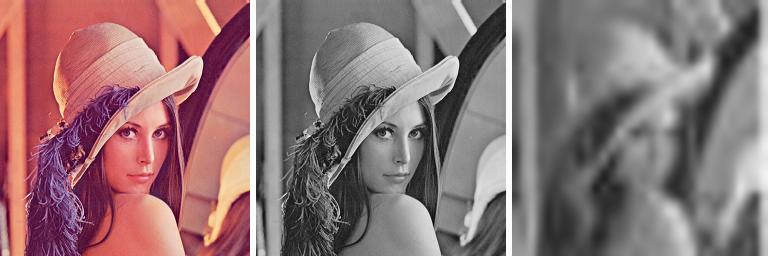
\includegraphics[scale=0.4]{Images/Lena.jpg}
		\caption{Approche naïve}
	\end{figure}
\end{frame}

\begin{frame}{Pooling}
	\begin{figure}[H]
		\centering
		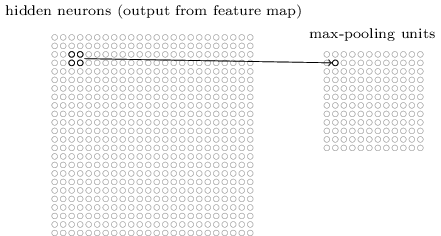
\includegraphics[scale=0.65]{Images/Pooling_Layer.png}
		\caption{\emph{Max-pooling} sur une fenêtre $(2,2)$}
	\end{figure}
\end{frame}

\begin{frame}{Images SpaceNet}
	\begin{table}[H]
		\centering
		\begin{tabular}{|c|c|}
		\hline 
		Résolution & WorldView-3 \\ 
		\hline 
		Bande Panchromatique & 0.31m \\ 
		\hline 
		Bandes Multispectrales (8) & 1.24m \\ 
		\hline
		\end{tabular}
		\caption{Résolution des capteurs optiques du satellite WorldView-3}	
	\end{table}
	\begin{table}[H]
		\centering
		 \begin{tabular}{|c|c|c|c|c|c|}
		\hline 
		Villes & Las Vegas & Paris & Shanghai & Khartoum & Total \\ 
		\hline 
		Images & 3851 & 1148 & 4582 & 1012 & 10593 \\ 
		\hline 
		Taille & 26.1Go & 7.8Go & 31.0Go & 6.8Go & 71.7Go \\ 
		\hline 
		\end{tabular}
		\caption{Distribution des images selon les différentes zones géographiques}
	\end{table} 
\end{frame}

\begin{frame}{Images SpaceNet (RGB, 8-bits, Correction $[2-98]\%$)}
	\begin{figure}[H]
		\centering
		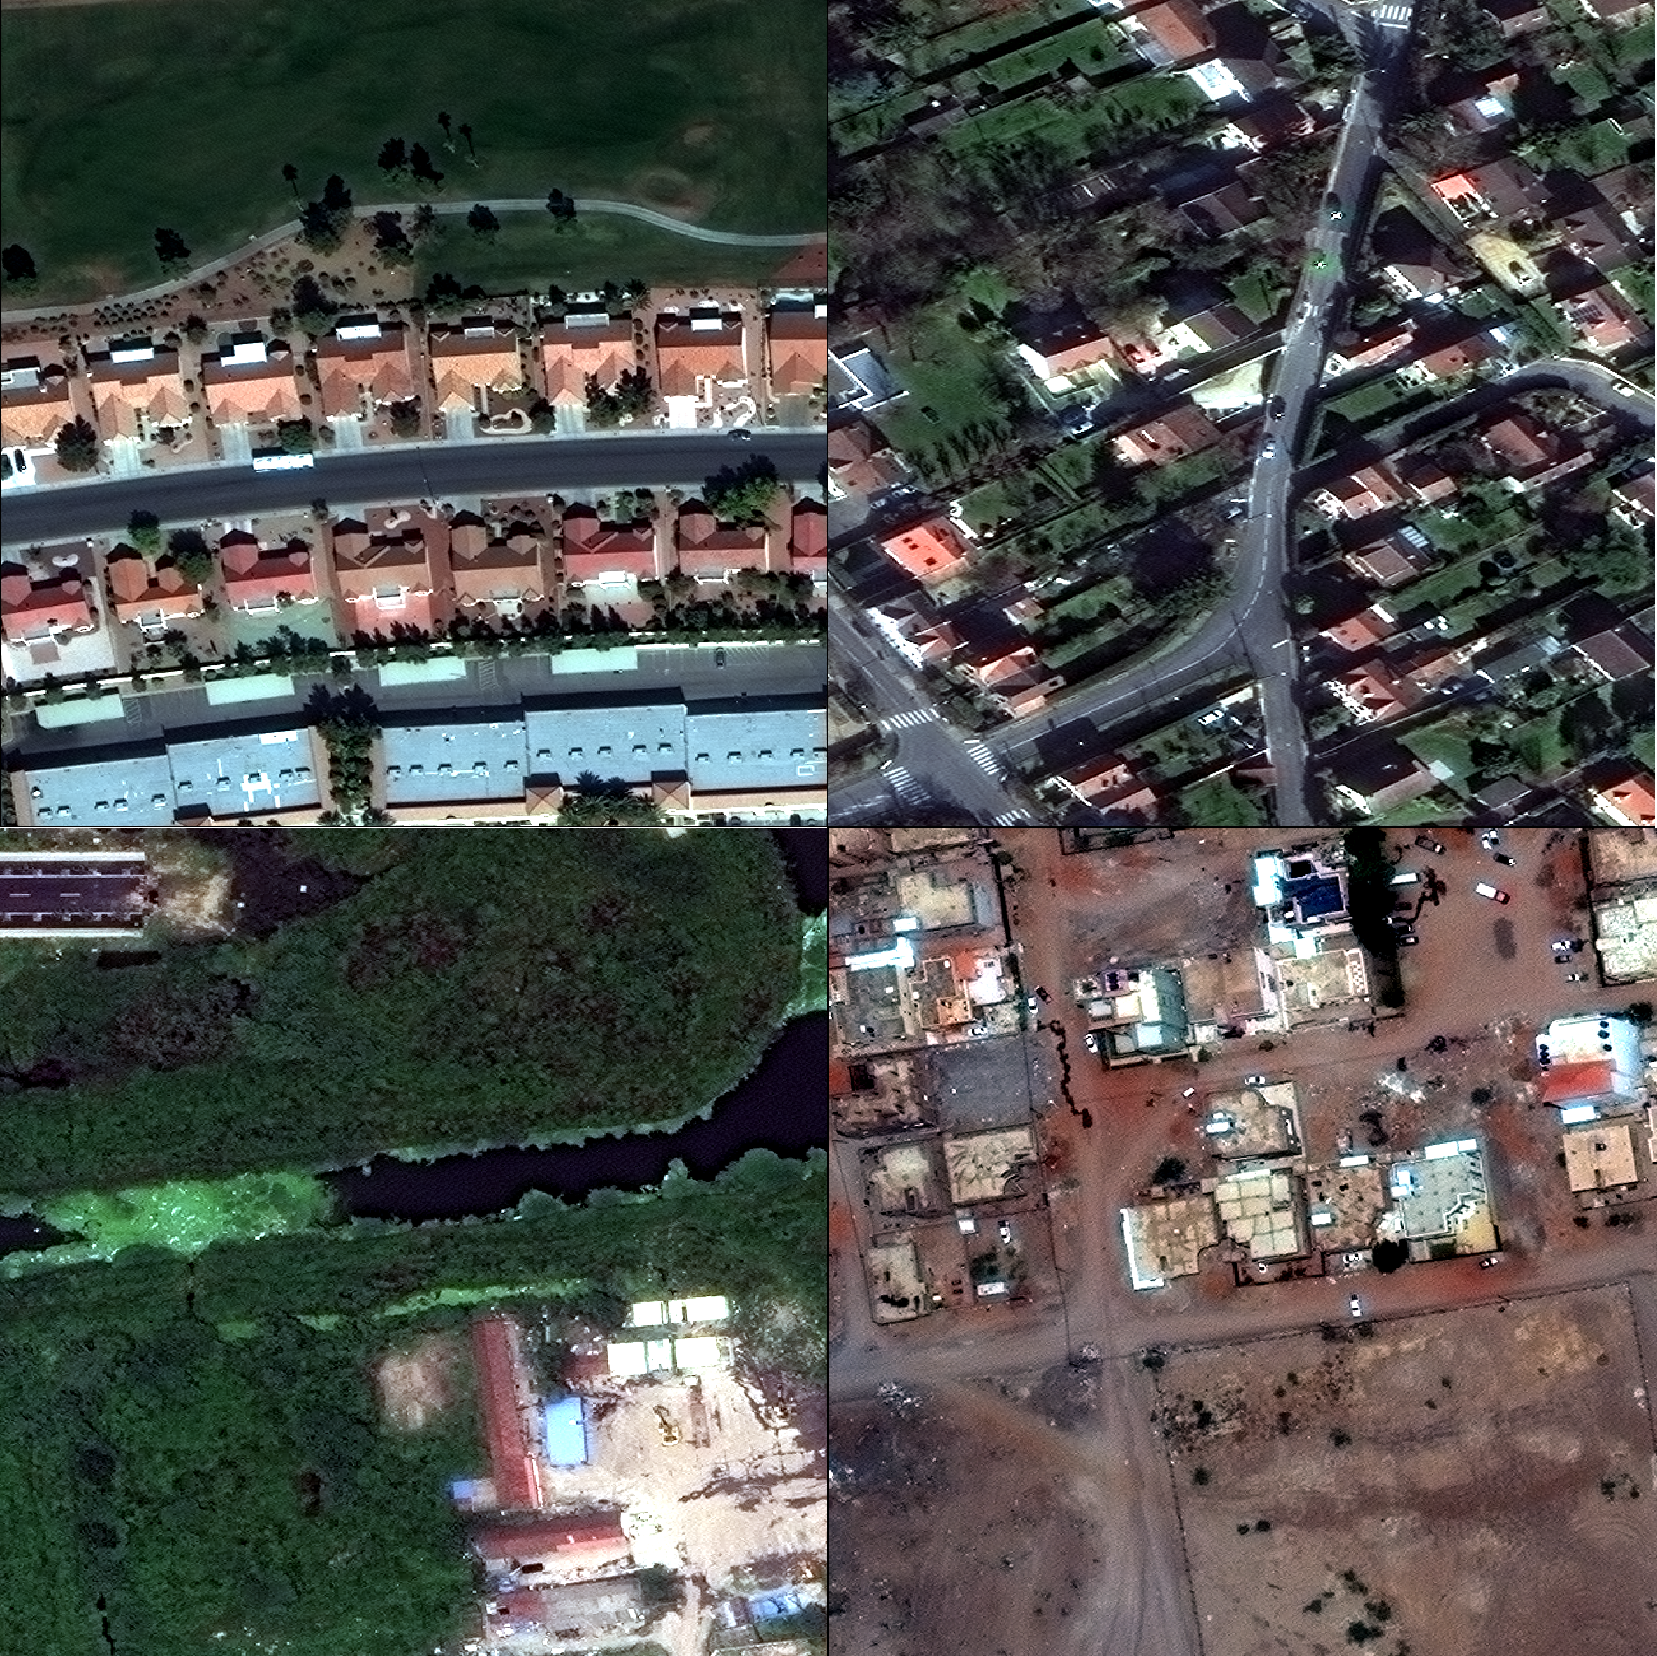
\includegraphics[scale=0.14]{Images/MUL_PAN.png}
	\end{figure}
\end{frame}

\begin{frame}[fragile]{Labels SpaceNet}
\begin{verbatim}
{
  "type": "FeatureCollection",
  "crs": {"type": "name",
    "properties": {"name": "urn:ogc:def:crs:1.3:CRS84"}},
  "features": [
    {	"geometry": {
        "type": "Polygon",
        "coordinates": [
            [-115.302252599989529, 36.208218543364502, 0.0],
            [-115.302260806999982, 36.208218603000034, 0.0]
            [...]]}
    }
[...]
}
\end{verbatim}
\end{frame}

\begin{frame}{Rasterisation des Labels de SpaceNet et d'OpenStreetMap}
	\begin{figure}[H]
		\centering
		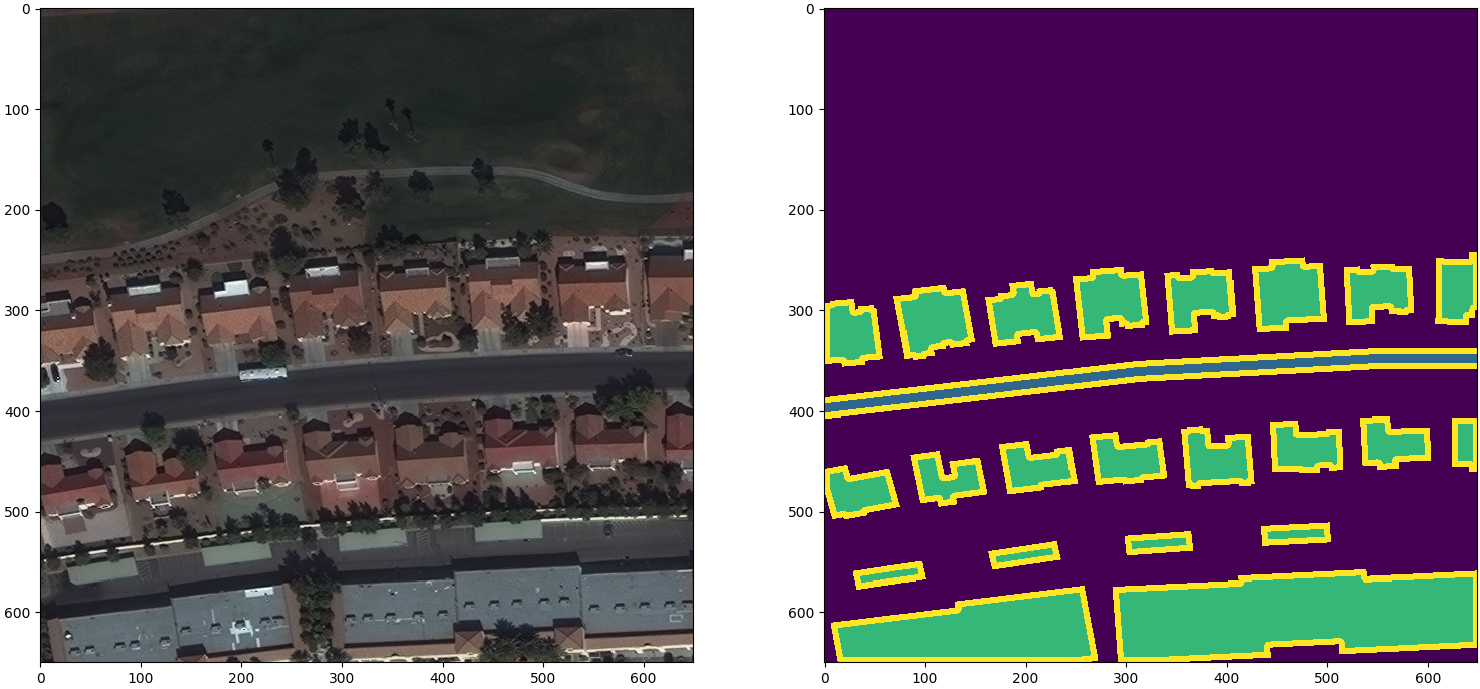
\includegraphics[scale=0.2125]{Images/MUL_PAN_Label_Vegas.png}
	\end{figure}
\end{frame}

\begin{frame}{CUDA et Caffe}
	\begin{block}{CUDA}
		Réseaux de neurones \emph{feedforward} sont totalement parallélisable.
		
		Calcul sur GPU environ 50 fois plus rapide que sur CPU.
	\end{block}
	\begin{block}{Caffe}
		Développé sous licence BSD par le \emph{Berkeley AI Research} et la communauté.

		Très utilisé en milieu académique.	
	\end{block}
\end{frame}

\begin{frame}{Unpooling}
	\begin{figure}[H]
		\centering
		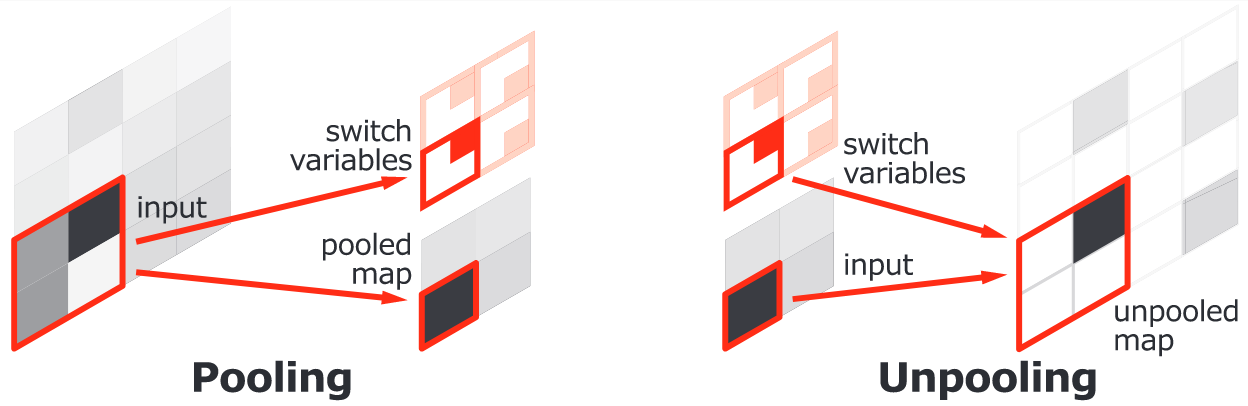
\includegraphics[scale=0.25]{Images/Unpooling.png}
		\caption{Couches de \emph{pooling} et d'\emph{unpooling}}
	\end{figure}
\end{frame}
\begin{frame}{Deconvolution}
	\begin{figure}[H]
		\centering
		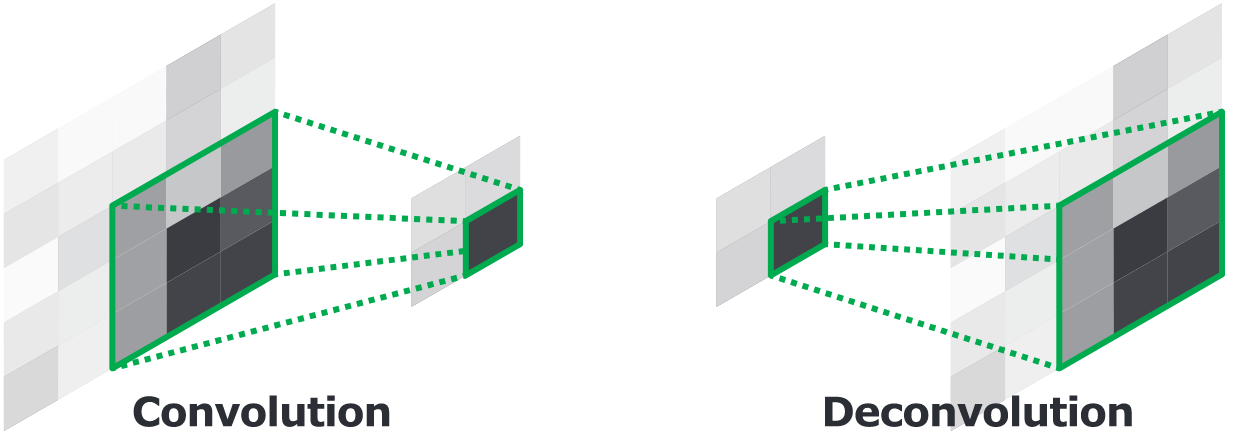
\includegraphics[scale=0.25]{Images/Deconvolution.png}
		\caption{Couches de convolution et de déconvolution}
	\end{figure}
\end{frame}
\begin{frame}
	\begin{figure}[H]
		\centering
		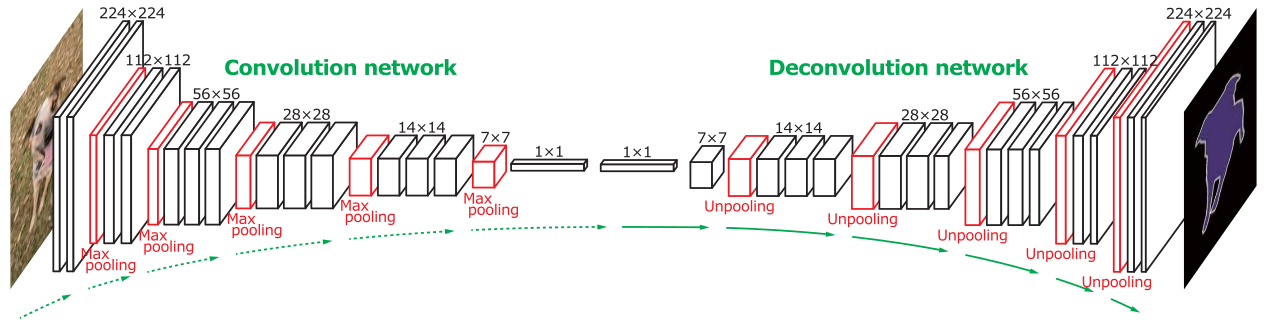
\includegraphics[scale=0.25]{Images/DeconvNet.png}
		\caption{Architecture DeconvNet}
	\end{figure}
\end{frame}

\begin{frame}{ZoomNet}
Architecture "allégée".

Utilisation de \emph{pooling} $(4, 4)$, et de convolutions $(3, 3)$ pour le bloc central.
\end{frame}
\begin{frame}{Courbes d'Apprentissage}
	\begin{figure}[H]
		\centering
		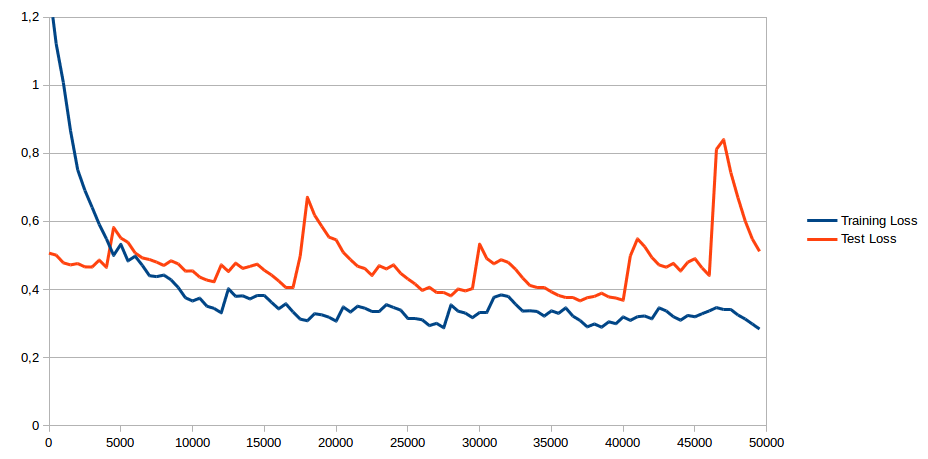
\includegraphics[scale=0.45]{Images/Losses_ZoomNet.png}
		\caption{Graphe de la fonction de perte pour le modèle ZoomNet}
	\end{figure}
\end{frame}
\begin{frame}{Analyse des Résultats}
	\begin{table}[H]
		\centering
		\begin{tabularx}{0.5\textwidth}{c|c c c|}
			Réel/Prédit & Bâtiment & Route & Absence \\
			\hhline{----}
			Bâtiment & 0.825 \cellcolor[gray]{.8} & \multicolumn{2}{c|}{0.175} \\
			Route & 0.262* & 0.738 \cellcolor[gray]{.8} & 0.262*\\
			Absence & \multicolumn{2}{c}{0.176} & 0.824 \cellcolor[gray]{.8}\\
			\hhline{~---}
		\end{tabularx}
		\caption{Matrice de confusion du modèle ZoomNet à l'itération 37000}
	\end{table}
\end{frame}

\begin{frame}{Inférence de ZoomNet}
	\begin{figure}[H]
		\centering
		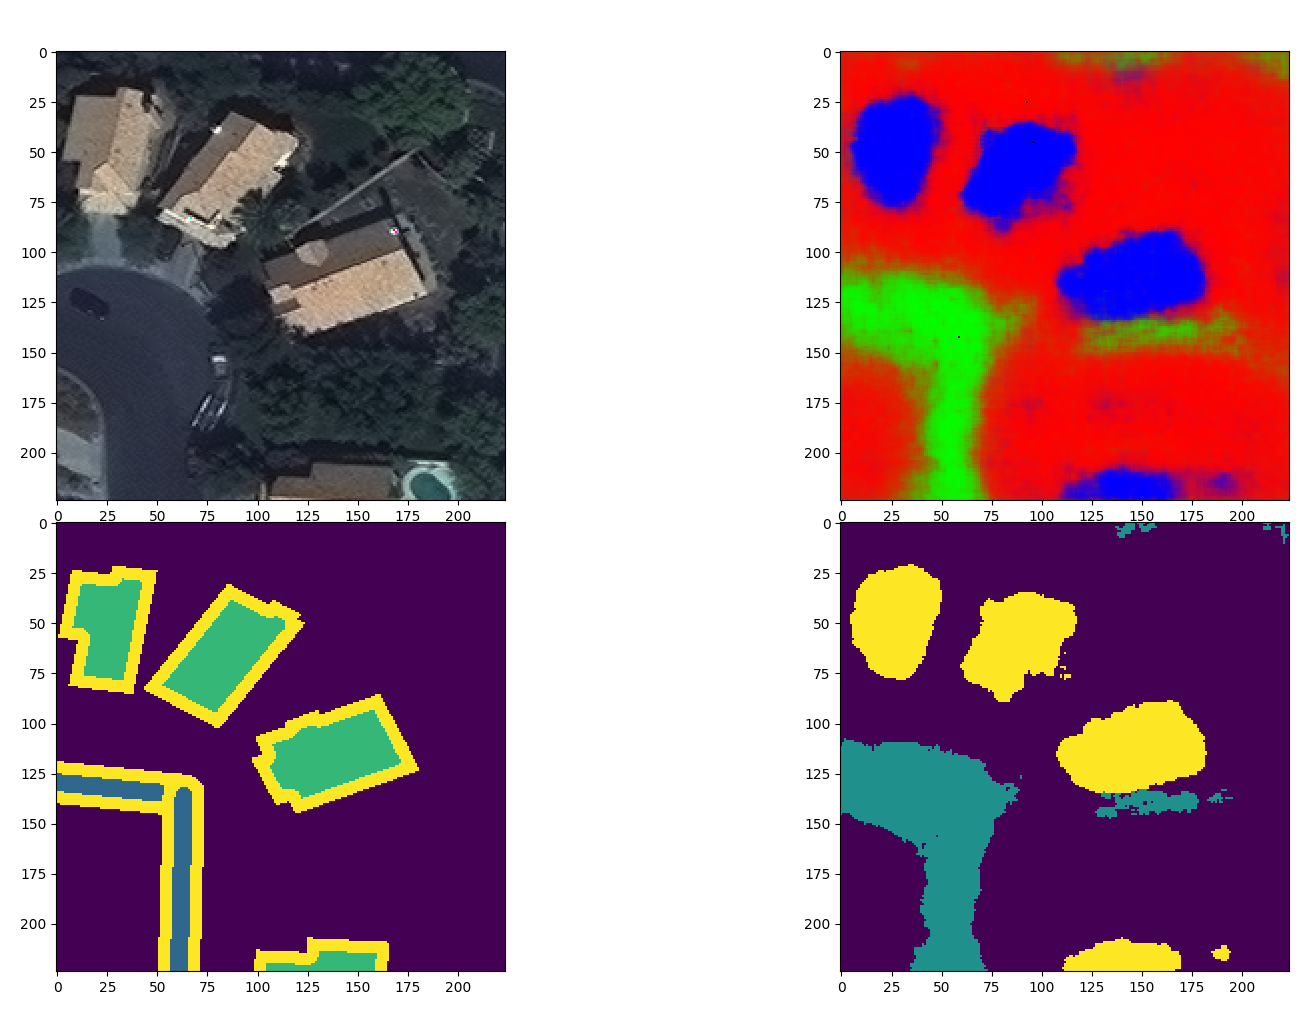
\includegraphics[scale=0.2]{Images/ZoomNet_1983.png}
	\end{figure}
\end{frame}

\begin{frame}{Inférence de ZoomNet}
	\begin{figure}[H]
		\centering
		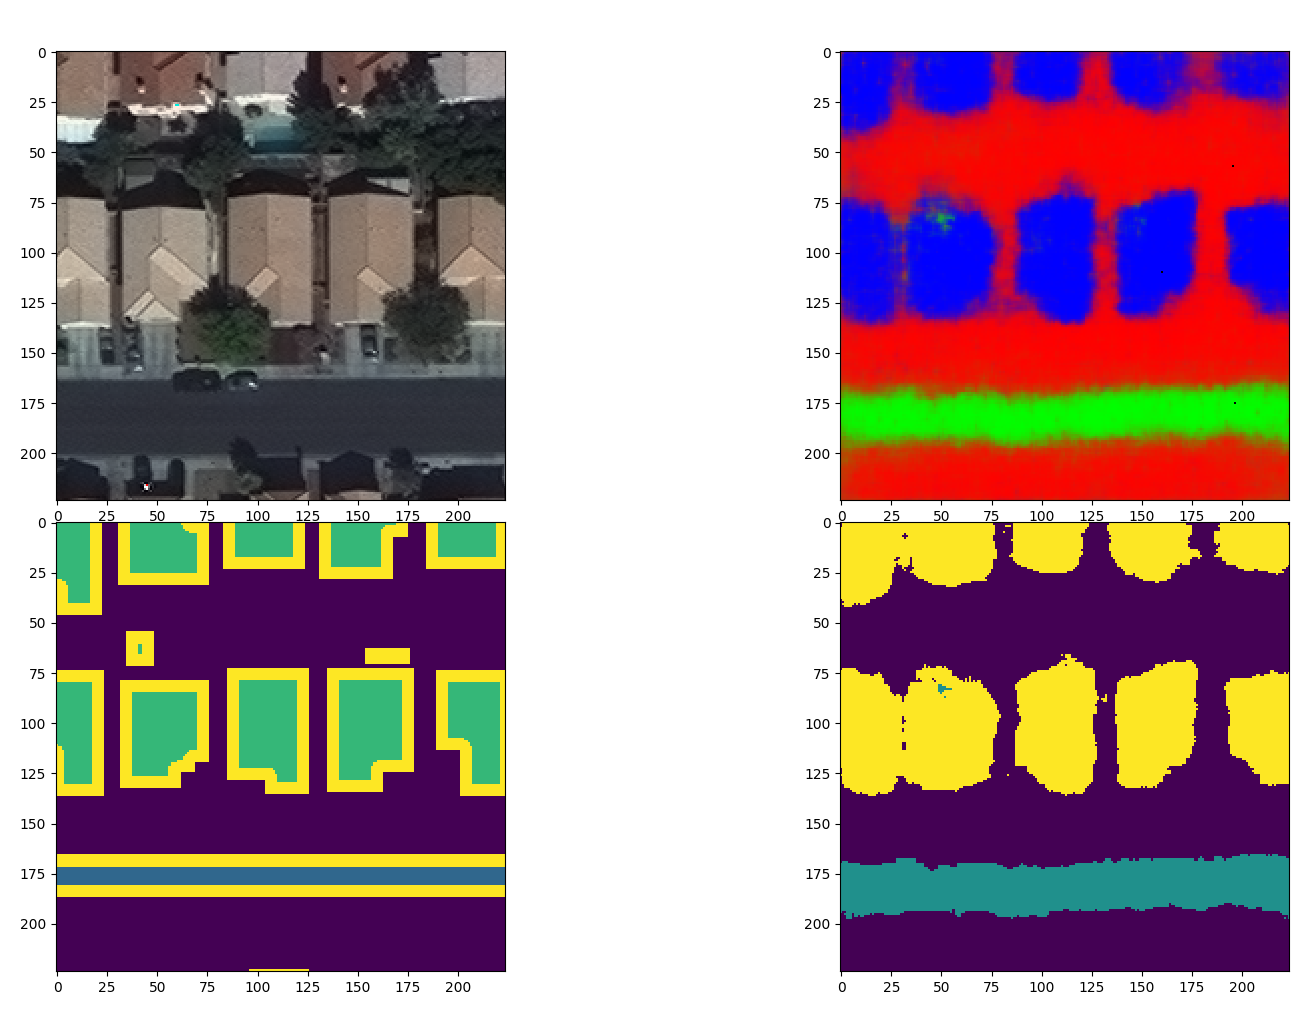
\includegraphics[scale=0.2]{Images/ZoomNet_5000.png}
	\end{figure}
\end{frame}

\begin{frame}{Classification Dynamique}
	Décomposition en trois étapes :
	\begin{enumerate}
		\item L'entraînement d'un modèle à une tâche de vision par ordinateur quelconque.
		\item La création semi-supervisée d'un \emph{dataset} de classification d'images.
		\item L'entraînement d'un second modèle à la classification d'images sur le \emph{dataset} précédemment créé.
	\end{enumerate}
\end{frame}

\begin{frame}{Commerce City (RGB, 8bits, Correction $[2-98]\%$)}
	\begin{figure}[H]
		\centering
		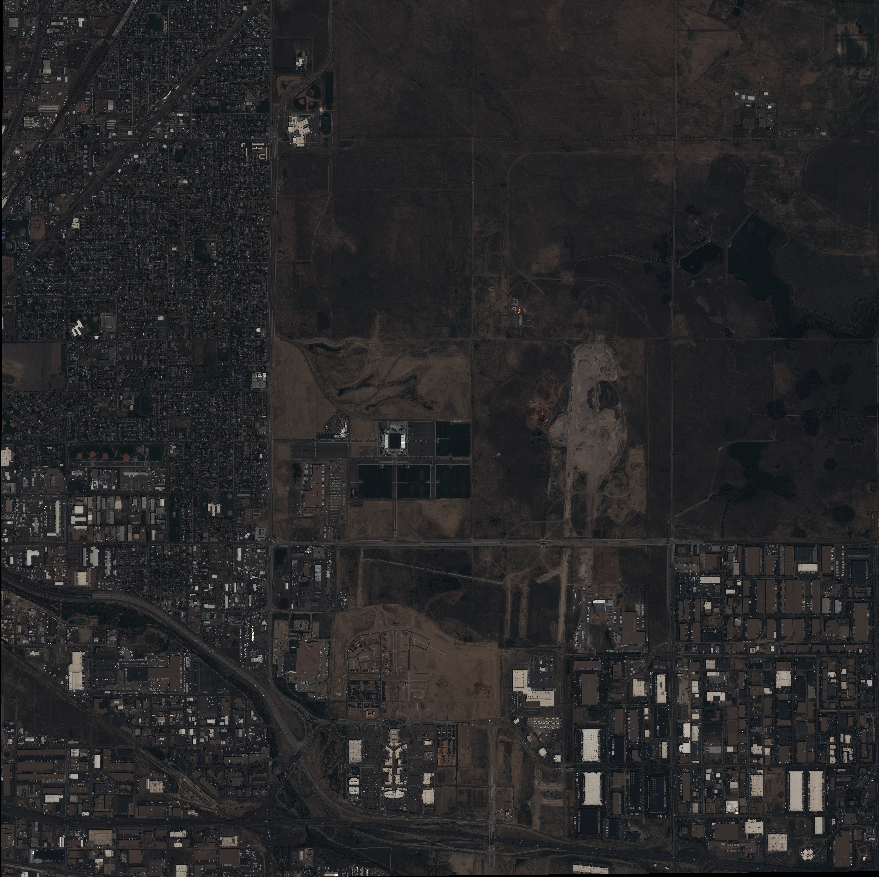
\includegraphics[scale=0.35]{Images/CommerceCity.png}
	\end{figure}
\end{frame}

\begin{frame}{Corrélation de \emph{patchs} décomposés en \emph{features}}
	\begin{figure}[H]
		\centering
		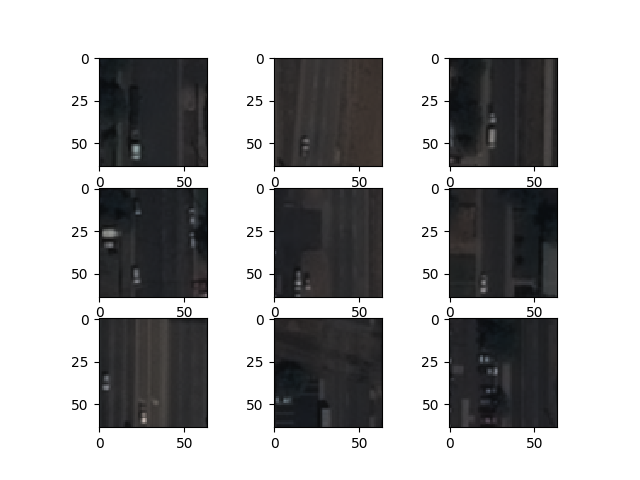
\includegraphics[scale=0.6]{Images/CommerceCity_Correlation_1.png}
	\end{figure}
\end{frame}

\begin{frame}{Corrélation de \emph{patchs} décomposés en \emph{features}}
	\begin{figure}[H]
		\centering
		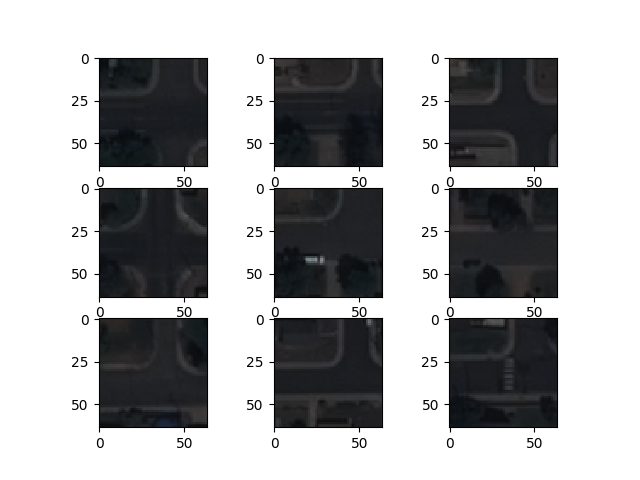
\includegraphics[scale=0.6]{Images/CommerceCity_Correlation_2.png}
	\end{figure}
\end{frame}

\begin{frame}{Conclusion}
	\begin{itemize}
		\item Sujet passionnant.
		\item Beaucoup d'autonomie.
		\item Souhait de poursuivre avec un doctorat dans le domaine de l'Apprentissage Profond.
	\end{itemize}
\end{frame}
\end{document}